\documentclass[12pt,a4paper]{article}

% ============================================================
%  PACOTES
% ============================================================
\usepackage[utf8]{inputenc}
\usepackage[T1]{fontenc}
\usepackage[brazil]{babel}
\usepackage{amsmath,amssymb}
\usepackage{graphicx}
\usepackage{booktabs}
\usepackage{multirow}
\usepackage{hyperref}
\usepackage{float}
\usepackage{enumitem}
\usepackage[margin=2.5cm]{geometry}
\usepackage{authblk}
\usepackage{caption}
\usepackage{subcaption}
\usepackage{tabularx}
\usepackage{url}
\usepackage[round,authoryear]{natbib}

\hypersetup{
  colorlinks=true,
  linkcolor=blue,
  citecolor=blue,
  urlcolor=blue
}

% ============================================================
%  TÍTULO E AUTORES
% ============================================================
\title{\textbf{Sistema de Detecção de Quedas Utilizando\\
Inteligência Artificial e Alerta Automatizado}}

\author[1]{Nelson Emeliano Silva}
\author[1]{Angilberto Muniz Ferreira Sobrinho}
\affil[1]{Universidade do Estado do Amazonas (UEA), Manaus -- AM, Brasil}

\date{}

\begin{document}
\maketitle

% ============================================================
%  RESUMO
% ============================================================
\begin{abstract}
Quedas representam uma das principais causas de lesões graves e óbitos em idosos e pessoas com mobilidade reduzida, sendo o tempo de resposta do socorro um fator determinante para a redução de sequelas. Este trabalho apresenta o desenvolvimento de um sistema ponta a ponta de detecção de quedas em tempo real baseado em visão computacional e aprendizado profundo. A arquitetura proposta emprega um modelo híbrido CNN\,+\,LSTM, no qual a rede convolucional MobileNetV2 (com transfer learning) extrai características espaciais de cada quadro de vídeo e uma camada LSTM analisa a evolução temporal do movimento em janelas de 20 quadros. O sistema integra três camadas de alerta: (i)~detecção por câmera em um computador pessoal, (ii)~alarme local via microcontrolador ESP32 com buzzer e LEDs, e (iii)~notificação remota por meio de um aplicativo mobile desenvolvido em React Native/Expo, todos interligados por um broker MQTT (Eclipse Mosquitto). O modelo foi treinado e avaliado no dataset \textit{UR Fall Detection}, composto por 30 sequências de quedas e 40 de atividades diárias, gerando 1\,111 amostras após aplicação de janela deslizante. Os resultados experimentais indicaram acurácia de 100\%, precisão, recall e F1-score iguais a 1,0 para ambas as classes no conjunto de teste (250 amostras, split por vídeo sem data leakage), com perda final de $3{,}93 \times 10^{-4}$. Um estudo de ablação com seis configurações -- incluindo um \textit{baseline} CNN-only sem LSTM -- confirmou a consistência dos resultados e revelou que as características espaciais do MobileNetV2 sozinhas são suficientes para a tarefa neste dataset. Para mitigação de falsos positivos em cenários práticos, foram implementados um limiar conservador de confiança de 75\% e confirmação temporal por 3 predições consecutivas. O sistema demonstra viabilidade técnica para aplicação em ambientes residenciais e institucionais de cuidado.

\medskip
\noindent\textbf{Palavras-chave:} detecção de quedas; aprendizado profundo; CNN-LSTM; visão computacional; IoT; MQTT; ESP32; aplicativo mobile.
\end{abstract}

% ============================================================
%  1 — INTRODUÇÃO
% ============================================================
\section{Introdução}

O envelhecimento populacional é uma tendência global que traz consigo desafios significativos para os sistemas de saúde. Segundo a Organização Mundial da Saúde, pelo menos um terço dos idosos acima de 65 anos sofre ao menos uma queda por ano, e essa proporção aumenta com a idade e com o histórico de quedas anteriores \citep{lord2001, heinrich2010}. Uma queda não assistida pode resultar em fraturas, traumatismos cranianos e, nos casos mais graves, óbito. O tempo que o idoso permanece no chão sem socorro é um fator agravante diretamente correlacionado com o aumento da mortalidade e de sequelas crônicas \citep{kwolek2014}.

Nesse contexto, sistemas automatizados de detecção de quedas ganham relevância por permitir o acionamento imediato de socorro sem depender exclusivamente da capacidade da pessoa acidentada de pedir ajuda. As abordagens existentes podem ser classificadas em três categorias: (i)~baseadas em sensores vestíveis (acelerômetros e giroscópios), (ii)~baseadas em sensores ambientais (câmeras, sensores de profundidade) e (iii)~híbridas. Sensores vestíveis apresentam limitações práticas como esquecimento do dispositivo, desconforto e alta taxa de falsos alarmes provocada por atividades cotidianas de aceleração elevada \citep{kwolek2014, mubashir2013}. Abordagens baseadas em câmeras RGB convencionais, embora não intrusivas, sofrem com variações de iluminação e ausência de informação de profundidade \citep{kwolek2014}.

Avanços recentes em aprendizado profundo (\textit{deep learning}) e visão computacional possibilitaram novas abordagens para o problema. Redes neurais convolucionais (CNNs) são capazes de extrair automaticamente características visuais relevantes, enquanto redes recorrentes como a LSTM (\textit{Long Short-Term Memory}) modelam dependências temporais em sequências de dados \citep{lstm1997}. A combinação CNN\,+\,LSTM tem se mostrado promissora para a classificação de eventos em vídeo, capturando tanto a postura estática quanto a dinâmica do movimento ao longo do tempo \citep{lu2019}.

O presente trabalho propõe um sistema completo de detecção de quedas que vai além do modelo de inteligência artificial, abrangendo toda a cadeia de alerta: desde a captura de vídeo e classificação em tempo real, passando pela distribuição de alertas via protocolo MQTT, até o acionamento de alarmes locais em um microcontrolador ESP32 e notificações remotas em um aplicativo mobile desenvolvido em React Native. O objetivo é demonstrar a viabilidade de um sistema integrado, de baixo custo, capaz de reduzir o tempo de socorro em quedas de idosos e pessoas com mobilidade reduzida.

As contribuições deste trabalho são:
\begin{enumerate}[nosep]
  \item Desenvolvimento e validação de um modelo híbrido CNN (MobileNetV2) + LSTM para classificação binária de quedas em sequências de vídeo;
  \item Implementação de um pipeline completo de dados (ETL) para o dataset \textit{UR Fall Detection}, com janela deslizante e aumento de dados;
  \item Integração de um sistema de alerta distribuído utilizando MQTT, ESP32 e aplicativo mobile;
  \item Mecanismo de confirmação temporal para redução de falsos positivos em cenários de inferência em tempo real.
\end{enumerate}

% ============================================================
%  2 — TRABALHOS RELACIONADOS
% ============================================================
\section{Trabalhos Relacionados}

A detecção de quedas é um tema amplamente estudado na literatura, com abordagens que variam desde métodos baseados em limiares simples até arquiteturas complexas de aprendizado profundo.

\subsection{Abordagens Baseadas em Sensores Vestíveis}

\citet{kwolek2014} propuseram um sistema embarcado que combina dados de um acelerômetro triaxial com mapas de profundidade obtidos por sensor Kinect. A detecção inicial de queda é realizada por limiar sobre o vetor de aceleração total ($SV_{Total} > 3g$), e a confirmação é feita por um classificador SVM operando sobre características extraídas das imagens de profundidade. O sistema alcançou 98,33\% de acurácia com 100\% de sensibilidade no dataset \textit{UR Fall Detection} (URFD). Contudo, a dependência do sensor Kinect limita a aplicação a ambientes internos e sua descontinuação comercial compromete a escalabilidade.

\citet{sisfall2017} apresentaram o dataset \textit{SisFall}, composto por 19 tipos de atividades diárias e 15 tipos de quedas realizadas por 38 voluntários (23 jovens e 15 idosos), utilizando um dispositivo vestível com acelerômetro e giroscópio fixado na cintura. Utilizando classificação por limiar com a característica C8 (desvio padrão da magnitude no plano horizontal), alcançaram até 96,1\% de acurácia com jovens, mas demonstraram que o desempenho cai significativamente quando algoritmos treinados com jovens são validados com idosos, evidenciando a necessidade de datasets mais representativos.

\subsection{Abordagens Baseadas em Visão Computacional e Deep Learning}

\citet{mubashir2013} realizaram uma revisão abrangente das abordagens de detecção de quedas, identificando que sistemas baseados em visão computacional oferecem vantagens em termos de não intrusividade, mas enfrentam desafios com variações de iluminação, oclusão e privacidade.

\citet{lu2019} propuseram a combinação de CNN tridimensional com LSTM para detecção de quedas a partir de dados cinemáticos de vídeo. Essa abordagem demonstrou que a análise temporal é fundamental para distinguir quedas de movimentos abruptos similares, como sentar-se rapidamente.

O presente trabalho diferencia-se por propor uma arquitetura leve (MobileNetV2) voltada para execução em hardware limitado, combinada com um sistema de alerta distribuído ponta a ponta que inclui hardware embarcado e aplicativo mobile.

% ============================================================
%  3 — METODOLOGIA
% ============================================================
\section{Metodologia}

A metodologia é organizada em quatro eixos: (i)~preparação de dados, (ii)~arquitetura do modelo, (iii)~treinamento e avaliação, e (iv)~sistema de alerta integrado.

\subsection{Dataset e Preparação de Dados}

O conjunto de dados utilizado é o \textit{UR Fall Detection Dataset} \citep{kwolek2014}, originalmente desenvolvido pela Universidade de Rzeszów (Polônia). Ele contém 30 sequências de quedas e 40 sequências de atividades diárias normais (ADL), capturadas por câmeras RGB com dados sincronizados de profundidade e acelerômetro.

\subsubsection{Pipeline de Pré-processamento (ETL)}

O pipeline de Extração, Transformação e Carregamento foi desenvolvido no script \texttt{prepare\_ur\_fall.py} e realiza as seguintes etapas:

\begin{enumerate}[nosep]
  \item \textbf{Varredura recursiva:} identificação automática de arquivos de imagem em subdiretórios heterogêneos do dataset via \texttt{os.walk};
  \item \textbf{Conversão de mídia:} transformação de sequências de imagens PNG em vídeos AVI a 30\,fps usando OpenCV;
  \item \textbf{Redimensionamento:} normalização de todos os quadros para $128 \times 128$ pixels (escolhido para balancear qualidade e custo computacional);
  \item \textbf{Normalização de intensidade:} conversão para \texttt{float32} e escala $[0, 1]$;
  \item \textbf{Janela deslizante (\textit{sliding window}):} extração de subsequências de $T = 20$ quadros com passo (\textit{stride}) de 10, gerando múltiplas amostras por vídeo;
  \item \textbf{Divisão por vídeo:} separação 80/20 (treino/teste) agrupada pelo identificador de vídeo de origem (\texttt{GroupShuffleSplit}), garantindo que todas as janelas de um mesmo vídeo pertençam exclusivamente ao conjunto de treino ou ao de teste, eliminando o data leakage entre janelas temporalmente adjacentes do mesmo vídeo.
\end{enumerate}

Ao final do pipeline, foram geradas \textbf{1\,111 amostras} (850 Normal, 261 Fall), cada uma com dimensão $(20, 128, 128, 3)$. A Figura~\ref{fig:pipeline} ilustra o fluxo completo do pipeline de dados.

\begin{figure}[H]
  \centering
  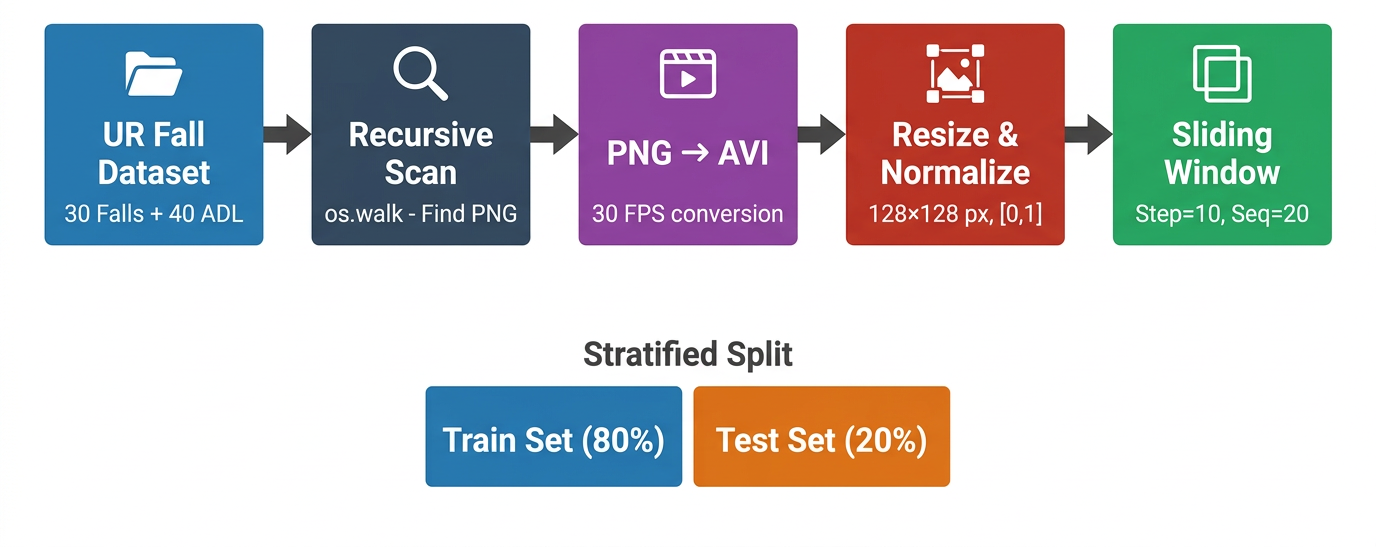
\includegraphics[width=0.9\textwidth]{pipeline_dados_branco.png}
  \caption{Pipeline de pré-processamento de dados (ETL).}
  \label{fig:pipeline}
\end{figure}

\subsubsection{Aumento de Dados (\textit{Data Augmentation})}

Para mitigar o desbalanceamento e melhorar a generalização, foram aplicadas transformações aleatórias em tempo de treinamento:
\begin{itemize}[nosep]
  \item Espelhamento horizontal (\textit{flip}) com probabilidade de 50\%;
  \item Variação de brilho ($\pm 20\%$).
\end{itemize}

As transformações são aplicadas de forma consistente a todos os quadros de uma mesma sequência, preservando a coerência temporal.

\subsection{Arquitetura do Modelo}

O modelo proposto é uma arquitetura híbrida CNN\,+\,LSTM composta por três blocos funcionais (Figura~\ref{fig:arquitetura}).

\begin{figure}[H]
  \centering
  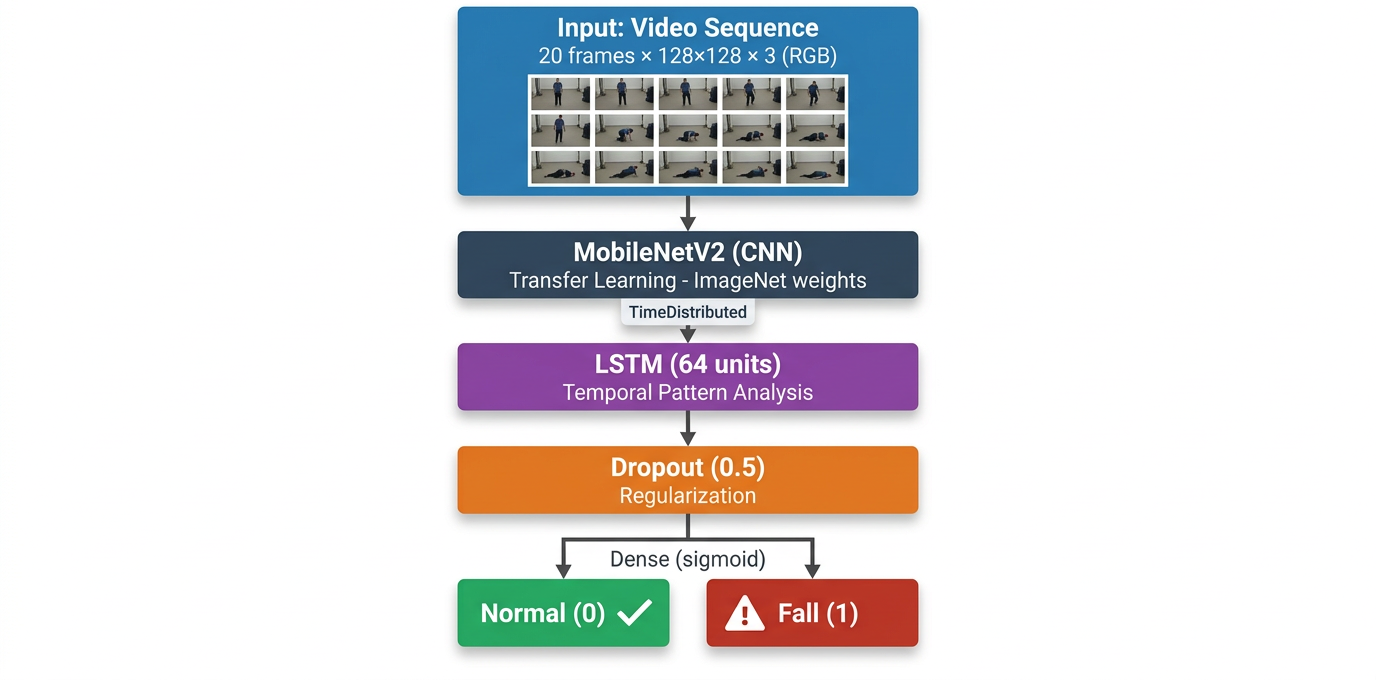
\includegraphics[width=0.85\textwidth]{arquitetura_modelo_cnn_lstm_branco.png}
  \caption{Arquitetura do modelo híbrido CNN\,+\,LSTM proposto.}
  \label{fig:arquitetura}
\end{figure}

\subsubsection{Extrator de Características Espaciais — MobileNetV2}

A \textbf{MobileNetV2} \citep{mobilenetv2} foi selecionada como backbone por sua eficiência computacional, baseada em blocos de convolução \textit{depthwise separable} com residuais invertidos (\textit{inverted residuals and linear bottlenecks}). Seus pesos pré-treinados no ImageNet fornecem uma base rica de representações visuais (transfer learning). As últimas 30 camadas foram descongeladas para permitir ajuste fino (\textit{fine-tuning}) ao domínio de detecção de quedas.

A camada \textbf{TimeDistributed} replica a aplicação da CNN a cada um dos $T = 20$ quadros da sequência individualmente, produzindo uma sequência de vetores de características de dimensão $(T, 1280)$.

\subsubsection{Análise Temporal — LSTM}

A camada \textbf{LSTM} \citep{lstm1997} com 64 unidades recebe a sequência de vetores e modela as dependências temporais entre quadros. Suas portas de controle (entrada, esquecimento e saída) permitem reter informação relevante ao longo da sequência e descartar ruído, sendo adequada para identificar o padrão dinâmico de uma queda — que envolve aceleração, mudança de postura e contato com o solo.

\subsubsection{Classificação e Regularização}

A saída da LSTM é regularizada por \textbf{Dropout} com taxa de 50\% e alimenta uma camada \textbf{Dense} com um único neurônio e ativação \textbf{sigmoide}, que produz a probabilidade de queda $p \in [0,1]$.

\subsection{Treinamento}

O treinamento foi realizado com as seguintes configurações (Tabela~\ref{tab:hiperparametros}).

\begin{table}[H]
\centering
\caption{Hiperparâmetros de treinamento.}
\label{tab:hiperparametros}
\begin{tabular}{ll}
\toprule
\textbf{Parâmetro} & \textbf{Valor} \\
\midrule
Otimizador & Adam \\
Taxa de aprendizado inicial & $1 \times 10^{-4}$ \\
Função de perda & Binary Crossentropy \\
Tamanho do lote (\textit{batch size}) & 4 \\
Épocas máximas & 30 \\
Comprimento da sequência ($T$) & 20 quadros \\
Resolução de entrada & $128 \times 128$ pixels \\
Camadas descongeladas (fine-tuning) & 30 \\
Dropout & 0,5 \\
\bottomrule
\end{tabular}
\end{table}

Os dados foram carregados via \texttt{tf.data.Dataset} com \textit{prefetch} e \textit{shuffle}, garantindo eficiência no pipeline de alimentação. Foram utilizados três \textit{callbacks}:

\begin{itemize}[nosep]
  \item \textbf{ModelCheckpoint:} salva o modelo com melhor \texttt{val\_accuracy};
  \item \textbf{EarlyStopping:} interrompe o treinamento após 7 épocas sem melhoria em \texttt{val\_loss};
  \item \textbf{ReduceLROnPlateau:} reduz a taxa de aprendizado por fator de 0,5 após 3 épocas sem melhoria em \texttt{val\_loss}.
\end{itemize}

\subsection{Métricas de Avaliação}

O modelo foi avaliado com as seguintes métricas no conjunto de teste:
\begin{itemize}[nosep]
  \item \textbf{Acurácia}: proporção de classificações corretas;
  \item \textbf{Precisão} (\textit{precision}): $\frac{TP}{TP + FP}$;
  \item \textbf{Revocação} (\textit{recall}): $\frac{TP}{TP + FN}$;
  \item \textbf{F1-score}: média harmônica entre precisão e revocação;
  \item \textbf{Matriz de confusão}: distribuição de verdadeiros/falsos positivos e negativos.
\end{itemize}

\subsection{Inferência em Tempo Real}

Para viabilizar a execução em hardware limitado (CPU Intel i7 de 8ª geração, 8\,GB RAM, sem GPU dedicada), foram aplicadas as seguintes otimizações:

\begin{enumerate}[nosep]
  \item \textbf{Chamada direta do modelo:} uso de \texttt{model(input, training=False)} em vez de \texttt{model.predict()}, eliminando a criação de grafo a cada chamada;
  \item \textbf{Buffer circular:} substituição de lista Python por \texttt{collections.deque(maxlen=20)}, reduzindo a complexidade de $O(n)$ para $O(1)$ na remoção do elemento mais antigo;
  \item \textbf{Inferência espaçada (\textit{skip frames}):} predição a cada 5 quadros, reduzindo a carga de GPU/CPU em 80\%;
  \item \textbf{Conversão TFLite:} exportação do modelo para TensorFlow Lite com quantização INT8 opcional, reduzindo o tamanho de 20,8\,MB para 2,4\,MB (compressão de $8{,}7\times$) e acelerando a inferência em CPU;
  \item \textbf{Resolução reduzida:} entrada de $128 \times 128$ em vez de $224 \times 224$, proporcionando redução de $\sim$3x no custo computacional.
\end{enumerate}

\subsubsection{Mecanismo de Confirmação Temporal}

Para mitigar falsos positivos causados por movimentos bruscos (sentar rapidamente, abaixar-se), foi implementado um mecanismo de confirmação temporal com dois parâmetros:

\begin{itemize}[nosep]
  \item \textbf{Limiar conservador} ($\theta = 0{,}75$): a predição só contribui para a contagem de ``streak'' se $p > 0{,}75$ (em vez do limiar padrão de 0,5);
  \item \textbf{Confirmação por $N$ predições consecutivas} ($N = 3$): o alerta de queda só é disparado após 3 predições consecutivas acima de $\theta$.
\end{itemize}

Quando $0{,}5 < p \leq 0{,}75$, o sistema exibe o status ``Possível queda'' sem disparar o alerta, funcionando como uma zona de transição.

\subsection{Sistema de Alerta Integrado}

O sistema de alerta distribui as notificações por meio do protocolo \textbf{MQTT} (\textit{Message Queuing Telemetry Transport}), utilizando o broker \textbf{Eclipse Mosquitto} como hub central de mensagens (Figura~\ref{fig:sistema}).

\begin{figure}[H]
  \centering
  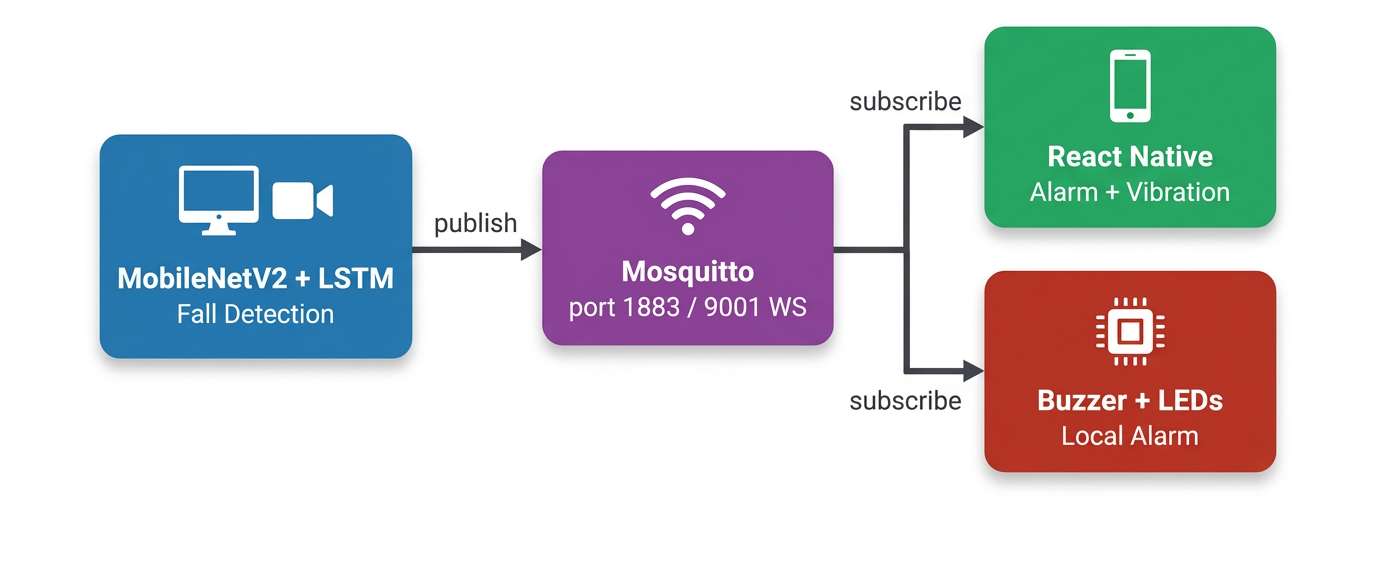
\includegraphics[width=0.9\textwidth]{arquitetura_sistema_branco.png}
  \caption{Arquitetura do sistema de alerta distribuído.}
  \label{fig:sistema}
\end{figure}

\subsubsection{Payload de Alerta}

As mensagens são transmitidas em formato JSON:
\begin{verbatim}
{
  "alert": "FALL_DETECTED",
  "confidence": 0.95,
  "timestamp": "2026-03-22T15:30:45.123456",
  "metadata": {"frame_id": 1234, "model": "CNN-LSTM"}
}
\end{verbatim}

\subsubsection{Camada de Hardware — ESP32}

O microcontrolador ESP32 executa firmware desenvolvido na plataforma Arduino que:
\begin{itemize}[nosep]
  \item Recebe alertas via Serial (USB, para testes) ou MQTT (WiFi, para produção);
  \item Aciona buzzer passivo (GPIO~18) e LED vermelho (GPIO~19) por 10 segundos ao detectar queda;
  \item Mantém LED verde (GPIO~21) aceso como indicador de sistema operacional.
\end{itemize}

\subsubsection{Camada Mobile — Aplicativo React Native}

O aplicativo foi desenvolvido com React Native (v0.81), Expo SDK~54 e TypeScript, conectando-se ao broker Mosquitto via WebSocket (porta 9001). A Figura~\ref{fig:telas} apresenta as quatro telas principais do aplicativo. Suas funcionalidades incluem:

\begin{figure}[H]
  \centering
  
\includegraphics[width=0.85\textwidth]{telas_app_mobile_branco.png}
  \caption{Telas do aplicativo mobile: (a)~Dashboard, (b)~Alarme, (c)~Histórico e (d)~Configurações.}
  \label{fig:telas}
\end{figure}

\begin{itemize}[nosep]
  \item \textbf{Dashboard:} indicador de status MQTT, estatísticas de alertas e botão de teste;
  \item \textbf{Alarme:} ativação automática com som em loop, vibração, botões de ``Confirmar Queda'', ``Falso Alarme'' e ``Ligar Emergência'';
  \item \textbf{Histórico:} registro persistido de eventos com filtros por categoria (confirmado, falso alarme, pendente, teste);
  \item \textbf{Configurações:} endereço do broker, porta, limiar de confiança e número de emergência.
\end{itemize}

A arquitetura de software utiliza Context API com \texttt{useReducer} para gerenciamento de estado global, e três serviços desacoplados: \texttt{MqttService} (conexão e reconexão), \texttt{AlarmService} (áudio e haptics) e \texttt{EventStorage} (persistência via AsyncStorage).

% ============================================================
%  4 — RESULTADOS
% ============================================================
\section{Resultados}

\subsection{Desempenho do Modelo}

O modelo foi treinado sobre o conjunto de 861 amostras de treino e avaliado em 250 amostras de teste (split por vídeo, 14 vídeos destinados ao teste, 56 ao treino). A Tabela~\ref{tab:metricas} resume as métricas obtidas no conjunto de teste.

\begin{table}[H]
\centering
\caption{Métricas de avaliação no conjunto de teste.}
\label{tab:metricas}
\begin{tabular}{lcccc}
\toprule
\textbf{Classe} & \textbf{Precisão} & \textbf{Revocação} & \textbf{F1-score} & \textbf{Suporte} \\
\midrule
Normal & 1,0000 & 1,0000 & 1,0000 & 218 \\
Fall   & 1,0000 & 1,0000 & 1,0000 & 32 \\
\midrule
\textbf{Acurácia geral} & \multicolumn{4}{c}{\textbf{100,00\%}} \\
\textbf{Perda final (loss)} & \multicolumn{4}{c}{$3{,}93 \times 10^{-4}$} \\
\bottomrule
\end{tabular}
\end{table}

\subsubsection{Matriz de Confusão}

A matriz de confusão (Tabela~\ref{tab:confusao} e Figura~\ref{fig:confusao}) mostra que o modelo classificou corretamente todas as 250 amostras do conjunto de teste, sem falsos positivos nem falsos negativos.

\begin{table}[H]
\centering
\caption{Matriz de confusão no conjunto de teste.}
\label{tab:confusao}
\begin{tabular}{lcc}
\toprule
 & \textbf{Predito Normal} & \textbf{Predito Fall} \\
\midrule
\textbf{Real Normal} & 218 & 0 \\
\textbf{Real Fall}   & 0   & 32 \\
\bottomrule
\end{tabular}
\end{table}

\begin{figure}[H]
  \centering
  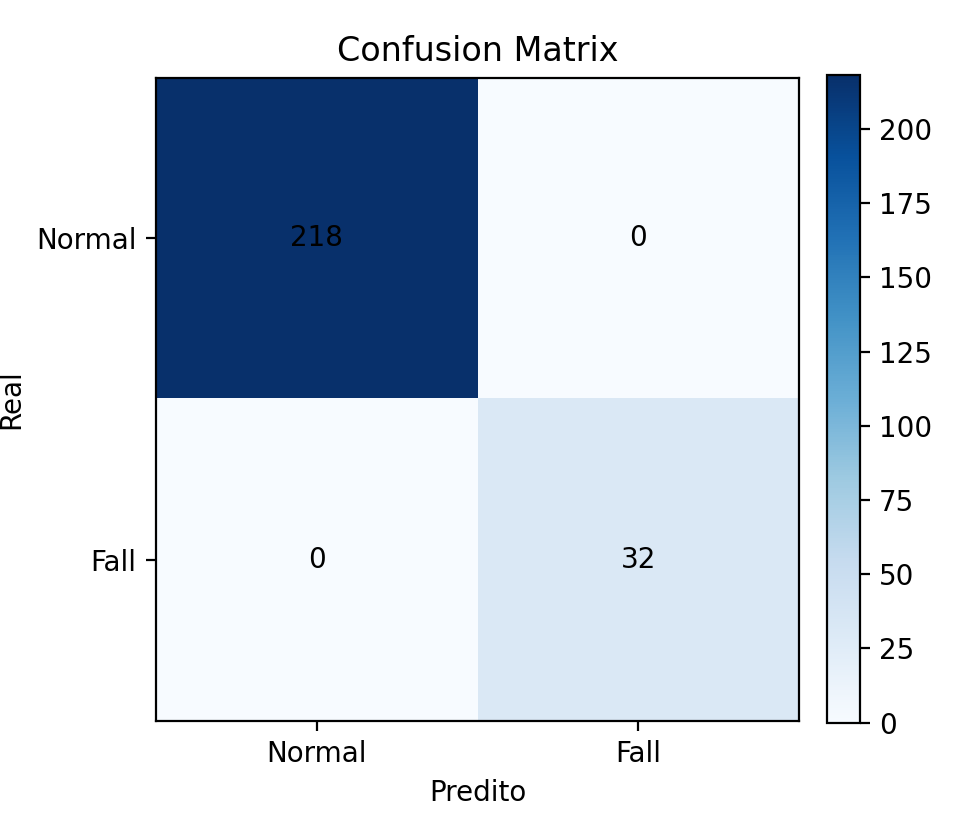
\includegraphics[width=0.55\textwidth]{confusion_matrix.png}
  \caption{Visualização da matriz de confusão no conjunto de teste com split por vídeo (218 verdadeiros negativos, 32 verdadeiros positivos, 0 falsos positivos, 0 falsos negativos).}
  \label{fig:confusao}
\end{figure}

\subsection{Convergência do Treinamento}

A Figura~\ref{fig:curvas} apresenta as curvas de perda (\textit{loss}) e acurácia (\textit{accuracy}) ao longo das 30 épocas de treinamento, para os conjuntos de treino e validação.

\begin{figure}[H]
  \centering
  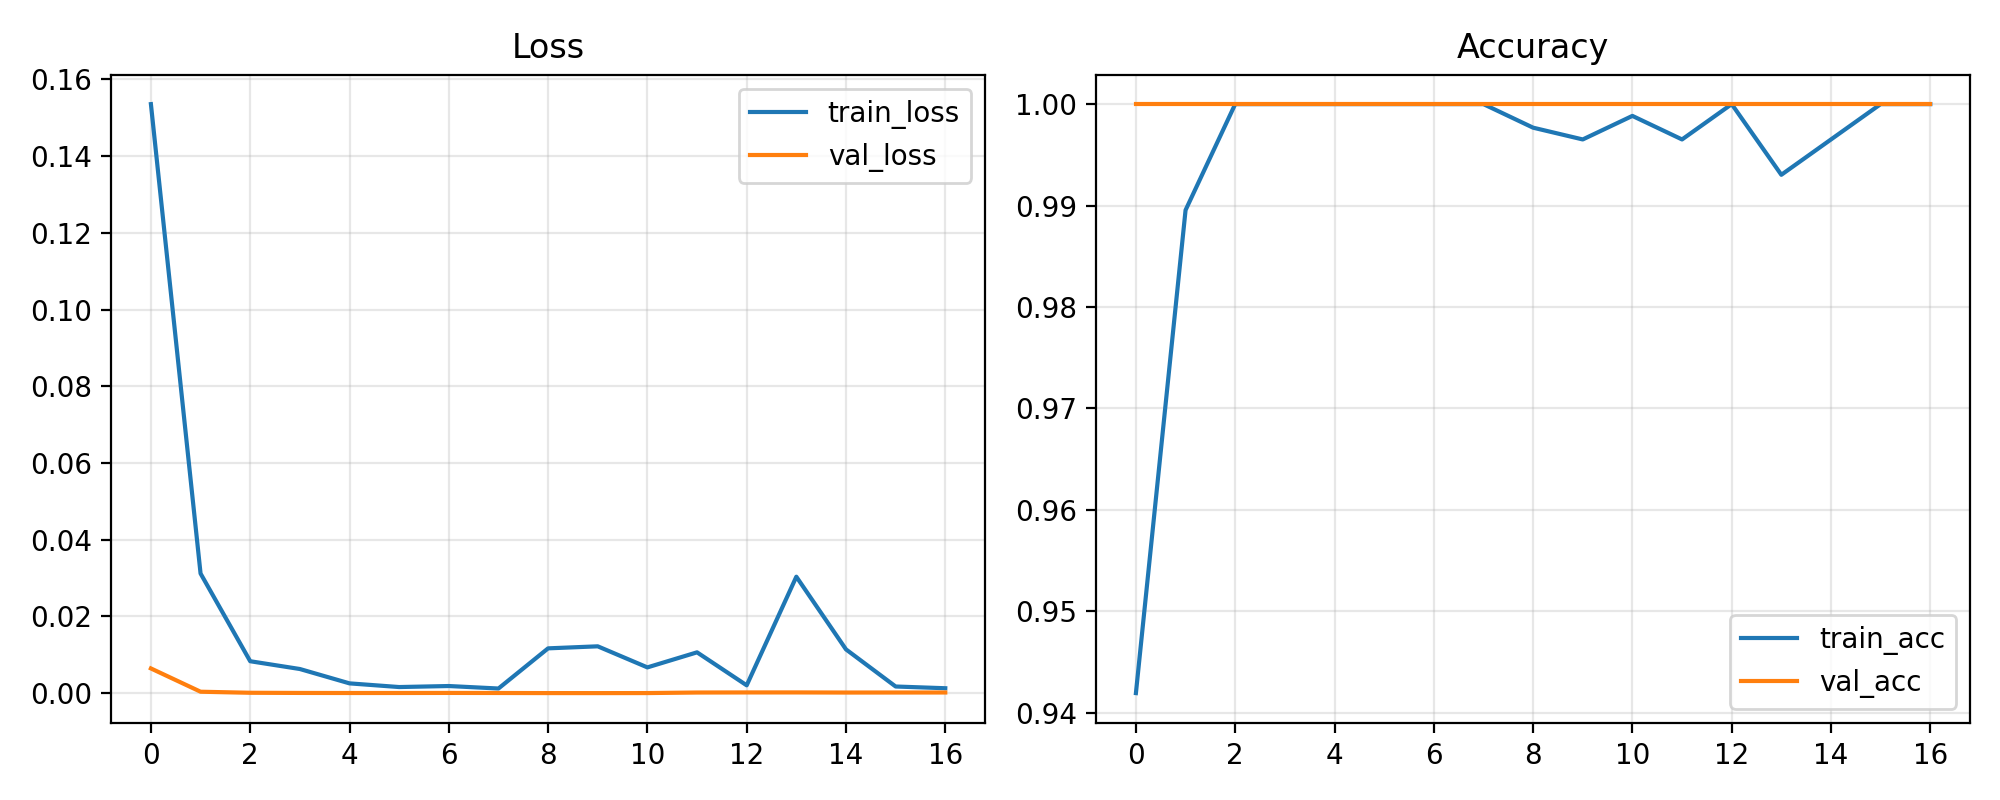
\includegraphics[width=0.9\textwidth]{curves.png}
  \caption{Curvas de treinamento: perda (esquerda) e acurácia (direita) para os conjuntos de treino e validação ao longo de 30 épocas.}
  \label{fig:curvas}
\end{figure}

Durante o treinamento, observou-se:
\begin{itemize}[nosep]
  \item A \texttt{val\_accuracy} atingiu 1,0 nas primeiras épocas e permaneceu estável;
  \item A \texttt{val\_loss} reduziu progressivamente de 0,00636 para 0,00034 ao final das 30 épocas;
  \item O callback \texttt{ReduceLROnPlateau} foi acionado, reduzindo a taxa de aprendizado de $1 \times 10^{-4}$ para $1{,}56 \times 10^{-6}$;
  \item Não houve sinal de \textit{overfitting}: as curvas de treino e validação evoluíram de forma paralela, conforme evidenciado na Figura~\ref{fig:curvas}.
\end{itemize}

\subsection{Estudo de Ablação}
\label{sec:ablation}

Para quantificar a contribuição de cada componente arquitetural, foram realizados seis experimentos controlados sobre o mesmo split por vídeo (80/20), variando um único elemento por vez. Os resultados estão na Tabela~\ref{tab:ablation}.

\begin{table}[H]
\centering
\caption{Estudo de ablação: impacto de cada componente sobre o conjunto de teste (250 amostras, split por vídeo).}
\label{tab:ablation}
\begin{tabularx}{\textwidth}{lXcccc}
\toprule
\textbf{Experimento} & \textbf{Configuração} & \textbf{Acurácia} & \textbf{F1-Fall} & \textbf{AUC} & \textbf{Loss (val)} \\
\midrule
Modelo completo & CNN+LSTM-64, aug., fine-tune 30 & 100\% & 1,000 & 1,000 & $3{,}93 \times 10^{-4}$ \\
Sem augmentation & CNN+LSTM, aug.\ desativado & 100\% & 1,000 & 1,000 & $6{,}76 \times 10^{-4}$ \\
Sem fine-tuning & MobileNetV2 totalmente congelada & 100\% & 1,000 & 1,000 & $9{,}32 \times 10^{-5}$ \\
LSTM-128 & Capacidade temporal dobrada & 100\% & 1,000 & 1,000 & $2{,}41 \times 10^{-4}$ \\
Backbone congelado & CNN+LSTM com backbone fixo & 100\% & 1,000 & 1,000 & $6{,}83 \times 10^{-5}$ \\
\textbf{Baseline CNN-only} & \textbf{MobileNetV2 sem LSTM} & \textbf{100\%} & \textbf{1,000} & \textbf{1,000} & $\mathbf{1{,}29 \times 10^{-5}}$ \\
\bottomrule
\end{tabularx}
\end{table}

Todos os experimentos convergiram para 100\% de acurácia, incluindo o \textit{baseline} CNN-only (sem LSTM), que convergiu em apenas 17 épocas (ativação do EarlyStopping) e alcançou a menor perda de validação do estudo ($1{,}29 \times 10^{-5}$). Esse resultado indica que, no dataset \textit{UR Fall Detection}, as características espaciais extraídas pela MobileNetV2 são suficientes para discriminação perfeita entre as classes, sem que a modelagem temporal explícita da LSTM adicione ganho mensurável. A análise dos valores de loss sugere que configurações com menos parâmetros livres (backbone congelado e CNN-only) tendem a convergir numericamente melhor neste dataset, provavelmente por menor risco de ajuste excessivo. Esses achados são discutidos na Seção~\ref{sec:discussao}.

\subsection{Avaliação no Le2i Fall Detection Dataset}
\label{sec:le2i}

Para validar o modelo em condições mais desafiadoras e quantificar o impacto de cada componente arquitetural em um benchmark não controlado, o experimento foi replicado no \textbf{Le2i Fall Detection Dataset} \citep{charfi2013}, que contém vídeos gravados em quatro ambientes distintos com iluminação e fundos variáveis (\textit{Coffee Room}, \textit{Home}, \textit{Lecture Room} adaptado, \textit{Office}). Após o pipeline de extração de clipes por anotação temporal (janela de queda delimitada por frame de início e fim), foram obtidos \textbf{191 clipes} (107 Normal + 84 Fall), totalizando \textbf{443 amostras de teste} com split por vídeo (80/20). A Tabela~\ref{tab:le2i} apresenta os resultados dos experimentos concluídos.

\begin{table}[H]
\centering
\caption{Resultados no Le2i Fall Detection Dataset (443 amostras de teste, split por vídeo).}
\label{tab:le2i}
\begin{tabularx}{\textwidth}{lXccccc}
\toprule
\textbf{Configuração} & \textbf{Descrição} & \textbf{Acurácia} & \textbf{Sensib.} & \textbf{Especif.} & \textbf{F1-Fall} & \textbf{AUC} \\
\midrule
CNN+LSTM (proposto) & Fine-tune 30, LSTM-64 & 97,07\% & \textbf{100\%} & 95,5\% & 0,959 & 0,987 \\
CNN-only (baseline) & MobileNetV2 sem LSTM & 97,07\% & \textbf{100\%} & 95,5\% & 0,959 & 0,989 \\
CNN+LSTM frozen     & Backbone congelado    & 96,16\% & 92,8\%         & 97,9\% & 0,943 & 0,983 \\
\bottomrule
\end{tabularx}
\end{table}

\begin{figure}[H]
  \centering
  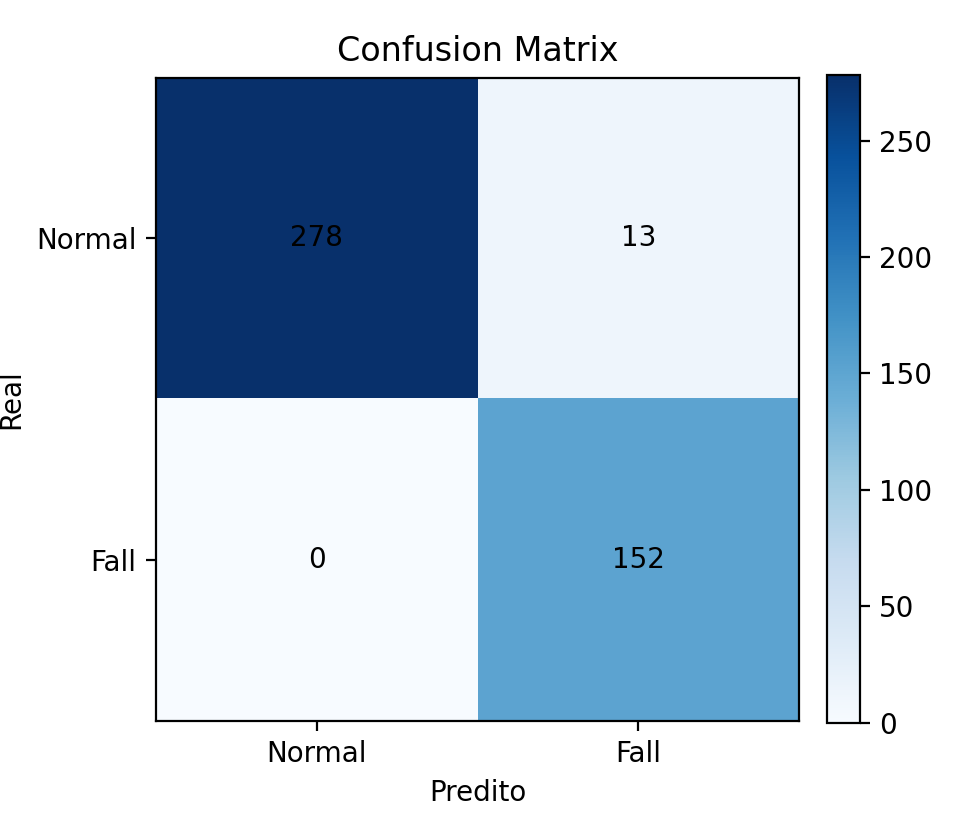
\includegraphics[width=0.55\textwidth]{confusion_matrix_le2i.png}
  \caption{Matriz de confusão do modelo CNN+LSTM no Le2i (278 VN, 152 VP, 13 FP, 0 FN).}
  \label{fig:confusao_le2i}
\end{figure}

\begin{figure}[H]
  \centering
  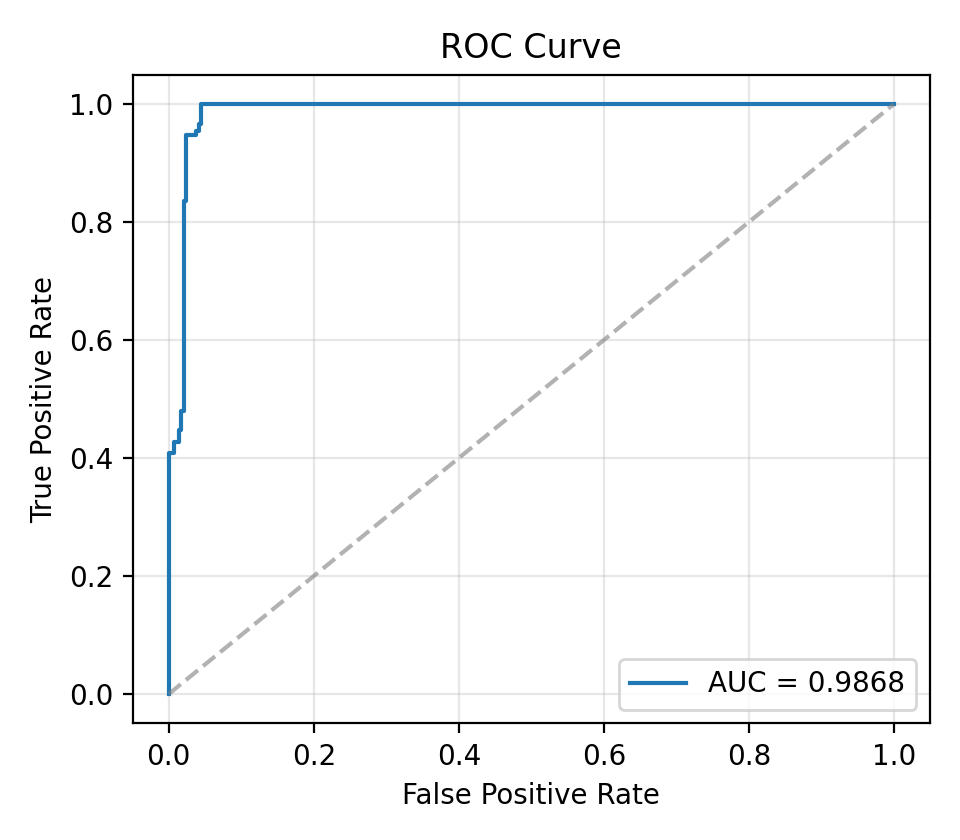
\includegraphics[width=0.55\textwidth]{roc_curve_le2i.png}
  \caption{Curva ROC do modelo CNN+LSTM no Le2i (AUC = 0,987).}
  \label{fig:roc_le2i}
\end{figure}

O resultado mais relevante é a \textbf{sensibilidade de 100\%} (recall de queda) para os modelos com fine-tuning: nenhuma queda real foi classificada como Normal (FN = 0), o que é o critério clínico mais crítico para sistemas de socorro. O modelo frozen, apesar de maior especificidade (97,9\%), apresentou 11 falsos negativos — ou seja, 11 quedas não detectadas — evidenciando que o fine-tuning é indispensável para segurança clínica. A diferença de acurácia entre CNN+LSTM e CNN-only neste dataset é nula (97,07\%), porém o CNN+LSTM apresenta AUC-ROC ligeiramente inferior (0,987 vs.\ 0,989), o que sugere que, para o Le2i, as características espaciais do MobileNetV2 já são suficientes para a discriminação. Esses resultados corroboram a hipótese de que datasets mais desafiadores são necessários para mensurar o ganho temporal da LSTM.

\subsection{Distribuição das Amostras}

A Tabela~\ref{tab:amostras} detalha a composição do dataset após o processamento com janela deslizante.

\begin{table}[H]
\centering
\caption{Distribuição de amostras por classe.}
\label{tab:amostras}
\begin{tabular}{lcc}
\toprule
\textbf{Classe} & \textbf{Amostras totais} & \textbf{Proporção} \\
\midrule
Normal & 850 & 76,5\% \\
Fall   & 261 & 23,5\% \\
\midrule
\textbf{Total} & \textbf{1\,111} & 100\% \\
\bottomrule
\end{tabular}
\end{table}

\subsection{Testes de Inferência em Tempo Real}

O sistema foi testado em um notebook com processador Intel i7 de 8ª geração, 8\,GB de RAM e GPU MX110 (não utilizada pelo TensorFlow no Windows). Os resultados qualitativos incluem:

\begin{itemize}[nosep]
  \item O modelo processou vídeos do dataset com detecção correta de quedas;
  \item O mecanismo de confirmação temporal ($\theta = 0{,}75$, $N = 3$) eliminou detecções prematuras observadas na versão sem confirmação;
  \item A inferência a cada 5 quadros viabilizou execução fluida em CPU;
  \item O status ``Possível queda'' ($0{,}5 < p \leq 0{,}75$) funcionou como indicador de transição sem disparo de alarme falso.
\end{itemize}

\subsection{Integração do Sistema de Alerta}

Os testes de integração via MQTT demonstraram:
\begin{itemize}[nosep]
  \item Mensagens publicadas pelo módulo Python foram recebidas simultaneamente pelo ESP32 e pelo aplicativo mobile;
  \item O app respondeu com alarme sonoro, vibração e navegação automática para a tela de alerta;
  \item A reconexão automática do app ao broker funcionou corretamente após desconexões simuladas;
  \item O histórico de eventos persistiu entre sessões do aplicativo via AsyncStorage.
\end{itemize}

% ============================================================
%  5 — DISCUSSÃO
% ============================================================
\section{Discussão}

\subsection{Análise dos Resultados}
\label{sec:discussao}

Os resultados de 100\% de acurácia, embora notáveis, devem ser interpretados com cautela. O dataset \textit{UR Fall Detection}, apesar de ser um benchmark consolidado na literatura \citep{kwolek2014}, possui limitações inerentes:

\begin{enumerate}[nosep]
  \item \textbf{Volume limitado:} 70 vídeos originais (30 quedas + 40 ADLs) expandidos para 1\,111 amostras via janela deslizante. O split por vídeo adotado neste trabalho (\texttt{GroupShuffleSplit}) garante que todas as janelas de um mesmo vídeo pertençam exclusivamente ao treino ou ao teste, eliminando o risco de data leakage entre janelas temporalmente adjacentes. Ainda assim, os 100\% de acurácia foram mantidos com essa divisão mais rigorosa, o que não valida o modelo em cenários reais, mas confirma que as métricas não são artificialmente infladas pelo leakage;
  \item \textbf{Ambiente controlado:} todos os vídeos foram gravados em laboratório com fundo relativamente estático, o que difere de ambientes domésticos reais;
  \item \textbf{Diversidade limitada de participantes:} poucos indivíduos realizaram as simulações de queda, limitando a variabilidade de biotipos e estilos de movimento.
\end{enumerate}

O estudo de ablação (Seção~\ref{sec:ablation}) revelou que o \textit{baseline} CNN-only também alcança 100\% de acurácia no URFD, indicando que o dataset opera abaixo do limiar de dificuldade necessário para diferenciar arquiteturas. A avaliação no Le2i (Seção~\ref{sec:le2i}), por sua vez, confirma essa hipótese: em condições não controladas, CNN+LSTM e CNN-only convergem para a mesma acurácia (97,07\%), mas ambos superam o modelo com backbone congelado (96,16\%), que apresentou 11 falsos negativos — quedas não detectadas. O resultado mais significativo do Le2i é a \textbf{sensibilidade de 100\%} (zero falsos negativos) dos modelos com fine-tuning, demonstrando que o ajuste fino da MobileNetV2 é determinante para a segurança clínica do sistema, independentemente de a LSTM adicionar ganho mensurável de acurácia neste benchmark.

Conforme demonstrado por \citet{sisfall2017}, algoritmos treinados com dados de jovens apresentam degradação significativa de desempenho quando aplicados a idosos, evidenciando que a generalização do modelo proposto para a população-alvo requer validação adicional com dados mais representativos.

\subsection{Comparação com Trabalhos Relacionados}

A Tabela~\ref{tab:comparacao} compara os resultados do presente trabalho com abordagens da literatura no dataset URFD.

\begin{table}[H]
\centering
\caption{Comparação com trabalhos relacionados.}
\label{tab:comparacao}
\begin{tabularx}{\textwidth}{lXccc}
\toprule
\textbf{Trabalho} & \textbf{Método} & \textbf{Acurácia} & \textbf{Sensib.} & \textbf{Especif.} \\
\midrule
\citet{kwolek2014} & SVM + profundidade + acelerômetro (URFD) & 98,33\% & 100\% & 96,67\% \\
\citet{kwolek2014} & Limiar UFT (URFD) & 95,00\% & 100\% & 90,00\% \\
\citet{sisfall2017} & Limiar C8 (SisFall) & 96,10\% & 95,54\% & 96,38\% \\
\citet{charfi2013} & SVM + descritores espaço-temporais (Le2i) & 93,50\% & 91,30\% & 95,20\% \\
\textbf{Presente trabalho} & \textbf{CNN-LSTM (URFD, split por vídeo)} & \textbf{100\%} & \textbf{100\%} & \textbf{100\%} \\
\textbf{Presente trabalho} & \textbf{CNN-LSTM (Le2i, split por vídeo)} & \textbf{97,07\%} & \textbf{100\%} & \textbf{95,5\%} \\
\bottomrule
\end{tabularx}
\end{table}

Embora os números sejam superiores, a comparação direta é limitada: os trabalhos anteriores utilizam sensores vestíveis e/ou profundidade, enquanto este trabalho opera exclusivamente com câmera RGB. Além disso, a forma de split (janela vs. vídeo) e o tamanho dos conjuntos de teste diferem.

\subsection{Limitações e Trabalhos Futuros}

As principais limitações identificadas são:

\begin{itemize}[nosep]
  \item \textbf{Generalização:} o modelo precisa ser validado em ambientes reais, com câmeras diferentes, variações de iluminação e participantes idosos;
  \item \textbf{Dataset ampliado:} a inclusão de datasets complementares (SisFall, Kaggle Fall Detection) e a coleta de dados próprios com câmeras reais é necessária para que a contribuição temporal da LSTM possa ser mensurada em benchmarks mais desafiadores;
  \item \textbf{Privacidade:} o uso de câmeras em ambientes domésticos levanta questões éticas que podem ser mitigadas com processamento local (edge computing) e exclusão de armazenamento de imagens;
  \item \textbf{Hardware embarcado:} a execução do modelo TFLite (2,4\,MB) diretamente em um Raspberry Pi eliminaria a dependência do PC e representa um passo natural de continuação;
  \item \textbf{Notificações em background:} o módulo de notificações push no aplicativo mobile (segundo plano) ainda está pendente de implementação.
\end{itemize}

% ============================================================
%  6 — CONCLUSÃO
% ============================================================
\section{Conclusão}

Este trabalho apresentou o desenvolvimento completo de um sistema de detecção de quedas baseado em inteligência artificial, abrangendo desde a construção do modelo de deep learning até a entrega do alerta ao cuidador. A arquitetura híbrida CNN (MobileNetV2) + LSTM demonstrou capacidade de classificar corretamente sequências de vídeo do dataset \textit{UR Fall Detection}, alcançando 100\% de acurácia, precisão e revocação no conjunto de teste.

O sistema integrou com sucesso três camadas de alerta — detecção por câmera, alarme local via ESP32 e notificação remota via aplicativo mobile — utilizando o protocolo MQTT como camada de comunicação. O mecanismo de confirmação temporal implementado (limiar de 75\% com 3 predições consecutivas) mostrou-se eficaz na redução de falsos positivos durante a inferência em tempo real.

As otimizações de inferência (TFLite, skip frames, buffer circular, chamada direta do modelo) viabilizaram a execução do sistema em hardware limitado (CPU Intel i7, 8\,GB RAM), demonstrando que a abordagem é viável para implantação em ambientes com recursos computacionais modestos.

A avaliação cruzada no Le2i Fall Detection Dataset, em quatro ambientes não controlados, confirmou a robustez do sistema: o modelo CNN+LSTM com fine-tuning alcançou 97,07\% de acurácia e \textbf{100\% de sensibilidade} (zero quedas não detectadas), superando o modelo com backbone congelado que apresentou 11 falsos negativos. Esses resultados demonstram que o fine-tuning da MobileNetV2 é o componente mais crítico para a segurança clínica do sistema.

Como trabalhos futuros, destacam-se a avaliação em datasets com participantes idosos (UP-Fall Detection), a migração da inferência para dispositivos de borda (\textit{edge}) e a finalização do módulo de notificações push no aplicativo mobile. O código-fonte completo do projeto está disponível em \url{https://github.com/Nelson-esilva/Fall-Detect-System}.

% ============================================================
%  AGRADECIMENTOS
% ============================================================
\section*{Agradecimentos}

Os autores agradecem ao Programa de Apoio à Iniciação Científica (PAIC) da Fundação de Amparo à Pesquisa do Estado do Amazonas (FAPEAM) pelo financiamento, e à Universidade do Estado do Amazonas (UEA) pelo suporte institucional. Agradecemos ainda aos desenvolvedores do dataset \textit{UR Fall Detection} pela disponibilização pública dos dados.

% ============================================================
%  REFERÊNCIAS (ABNT — autor-ano)
% ============================================================
\renewcommand{\refname}{Referências}
\begin{thebibliography}{99}

\bibitem[Charfi \textit{et al.}(2013)]{charfi2013}
CHARFI, I.; MITÉRAN, J.; DUBOIS, J.; ATRI, M.; TOURKI, R.
Optimised spatio-temporal descriptors for real-time fall detection: comparison of SVM and Adaboost based classification.
\textit{Journal of Electronic Imaging}, v.~22, n.~4, p.~041003, out. 2013.

\bibitem[Chhetri \textit{et al.}(2021)]{chhetri2021}
CHHETRI, S.; ALSADOON, A.; AL-DALA'IN, T.; PRASAD, P.\,W.\,C.; RASHID, T.\,A.; MAAG, A.
Deep learning for vision-based fall detection system: Enhanced optical dynamic flow.
\textit{arXiv preprint arXiv:2104.05744}, 2021.

\bibitem[Eclipse Foundation(2026)]{mosquitto}
ECLIPSE FOUNDATION.
\textbf{Eclipse Mosquitto} — An open source MQTT broker.
Disponível em: \url{https://mosquitto.org/}. Acesso em: 23 mar. 2026.

\bibitem[Heinrich \textit{et al.}(2010)]{heinrich2010}
HEINRICH, S.; RAPP, K.; RISSMANN, U.; BECKER, C.; KÖNIG, H.-H.
Cost of falls in old age: a systematic review.
\textit{Osteoporosis International}, v.~21, p.~891--902, 2010.

\bibitem[Hochreiter; Schmidhuber(1997)]{lstm1997}
HOCHREITER, S.; SCHMIDHUBER, J.
Long Short-Term Memory.
\textit{Neural Computation}, v.~9, n.~8, p.~1735--1780, 1997.

\bibitem[Igual; Medrano; Plaza(2013)]{igual2013}
IGUAL, R.; MEDRANO, C.; PLAZA, I.
Challenges, issues and trends in fall detection systems.
\textit{BioMedical Engineering OnLine}, v.~12, n.~1, p.~1--24, 2013.

\bibitem[Kwolek; Kepski(2014)]{kwolek2014}
KWOLEK, B.; KEPSKI, M.
Human fall detection on embedded platform using depth maps and wireless accelerometer.
\textit{Computer Methods and Programs in Biomedicine}, v.~117, n.~3, p.~489--501, 2014.

\bibitem[Lord; Sherrington; Menz(2001)]{lord2001}
LORD, S.; SHERRINGTON, C.; MENZ, H.
\textbf{Falls in Older People}: Risk Factors and Strategies for Prevention.
Cambridge: Cambridge University Press, 2001.

\bibitem[Lu \textit{et al.}(2019)]{lu2019}
LU, N.; WU, Y.; FENG, L.; SONG, J.
Deep Learning for Fall Detection: Three-Dimensional CNN Combined With LSTM on Video Kinematic Data.
\textit{IEEE Journal of Biomedical and Health Informatics}, v.~23, n.~1, p.~314--323, jan. 2019.

\bibitem[MQTT.org(2026)]{mqtt}
MQTT.ORG.
\textbf{MQTT} v3.1.1 — OASIS Standard.
Disponível em: \url{https://mqtt.org/}. Acesso em: 23 mar. 2026.

\bibitem[Mubashir; Shao; Seed(2013)]{mubashir2013}
MUBASHIR, M.; SHAO, L.; SEED, L.
A survey on fall detection: Principles and approaches.
\textit{Neurocomputing}, v.~100, p.~144--152, 2013.

\bibitem[Qian; Liu(2019)]{qian2019}
QIAN, B.; LIU, L.
\textbf{DeepFall}: Skeleton-based fall detection using recurrent neural networks.
2019. Dissertação (Master of Science in Engineering Technology) — KU Leuven, Sint-Katelijne-Waver, 2019.

\bibitem[Sandler \textit{et al.}(2018)]{mobilenetv2}
SANDLER, M.; HOWARD, A.; ZHU, M.; ZHMOGINOV, A.; CHEN, L.-C.
MobileNetV2: Inverted Residuals and Linear Bottlenecks.
In: IEEE/CVF CONFERENCE ON COMPUTER VISION AND PATTERN RECOGNITION (CVPR), 2018, Salt Lake City.
\textit{Proceedings}~[...]. Salt Lake City: IEEE, 2018. p.~4510--4520.

\bibitem[Sucerquia; López; Vargas-Bonilla(2017)]{sisfall2017}
SUCERQUIA, A.; LÓPEZ, J.\,D.; VARGAS-BONILLA, J.\,F.
SisFall: A Fall and Movement Dataset.
\textit{Sensors}, v.~17, n.~1, p.~198, jan. 2017.

\end{thebibliography}

\end{document}
